\chapter{Reward shaping for meta-learning}
\begin{quotation}
\noindent ``\emph{quote}''
\begin{flushright}\textbf{author}\end{flushright}
\end{quotation}


We have described in section \ref{section:problems_1_timestep_reward} why
a 1-per-timestep reward structure led to an undesired behaviour of laziness,
in which the agent only maximised its reward on the last episode of its
training trials.\\

We introduce a simple, yet effective way to allow problems with similar 
reward structures to be meta-learned. In hand-designed strategies aimed to
solve such problems, the designer holds the implicit knowledge that a short
episode is a bad thing, and treats the reward streams of each episode 
separately. In meta-learning, just like we feed back a termination flag, which
is not an environment-level value but rather a "process-level" value (where
the process is the training process we replicate in a trial); we can
introduce a process-level reward to give information to the agent 
performing the trial.\\

We propose to add a small negative reward at the end of each episode, 
interrupting the continuous reward stream to force the agent to perform
well for each of the episodes in the trial.\\

Our agent is trained on the training set of 20 permutations listed on table
\ref{tab:20perms}, on trials of 3 episodes. The reward for the last 
timestep of each episode is set to -10. Figure \ref{fig:magic} shows how
the episode-wise reward curve evolves during training. We see that all
three episodes reach a high reward, but more importantly, performance
increases for the second and third episode. \\

\begin{figure}
	\centering
	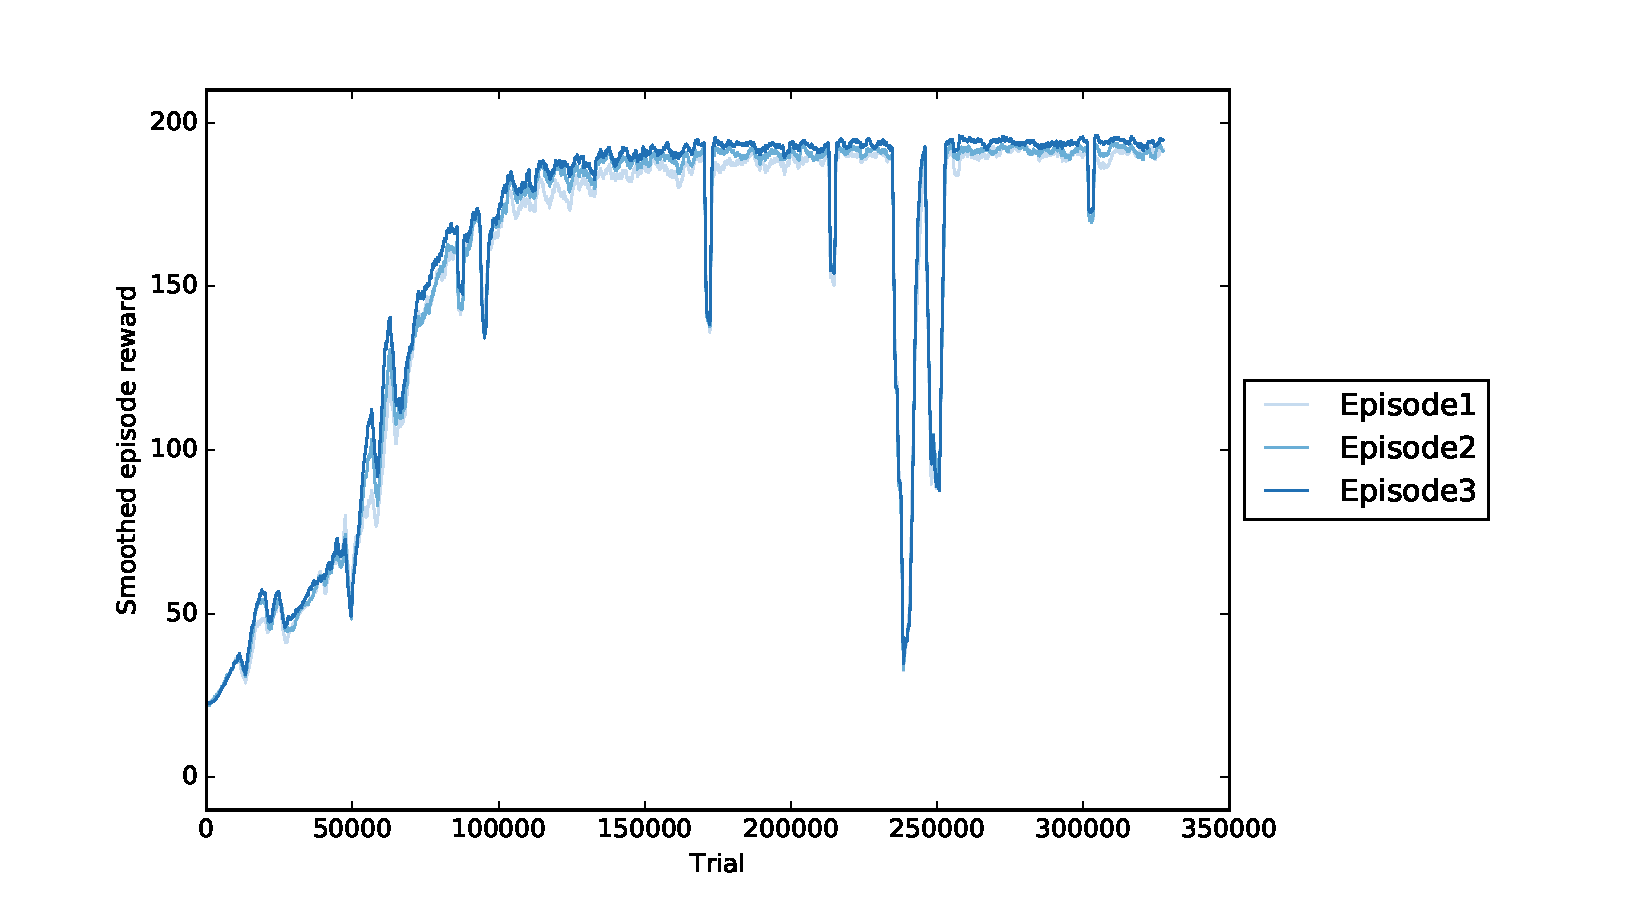
\includegraphics[width=0.8\linewidth]{fig/res_magic_neg10.pdf}
	\caption{Episode-wise reward evolution during the training of an
	agent playing trials of 3 episodes with a small negative reward
	at the end of each episode.}
	\label{fig:magic}
\end{figure}

\todo{histogram per episode}

Even though this is a success, we think there might be a better solution for
problems with a similar reward structure. For example, Wang et al.
\cite{learningtorl} present an experiment (bandits with dependent arms II) 
where the optimal long-term strategy is to start by playing a suboptimal action
voluntarily to gain information that will then allow the agent to play
optimal moves in future episodes. We believe our method doesn't allow for 
this voluntary payment in short-term reward; instead it will greedily try
to perform as well as it can by passing information from one episode to the
next.\\

We suspect that adapting the architecture presented by Wang et al. to allow
the outer algorithm to have knowledge of total episode rewards, instead of
timestep-only rewards could lead to an overall better learning algorithm.


